\chapter{SPARSE BAYESIAN LINEAR AND NONLINEAR MODELS ESTIMATED FOR SHORT-TERM FORECASTING OF TRAFFIC OCCUPANCY}
\label{chap:traffic}
%%%%%%%%%%%%%%%%%%%%%%%%%%%%%%%%%%%%%%%%%%%%%%%%%%%%%%%%%%%%%%%%%%%%%%%
\section{INTRODUCTION}
Rising populations in major cities add stress to advanced traffic management systems (ATMS) tasked with monitoring real-time traffic variables to proactively reduce congestion. Ever since \cite{Ahmed1979} used basic ARIMA strategies to model freeway traffic networks in large US cities -- Los Angeles, Minneapolis, and Detroit -- significant research has accumulated to appropriately utilize the massive amount of data obtained in transportation networks. The global concern has manifested through independent research in major cities in places such as the United Kingdom \citep{Queen2009,Dunne2012}, Greece \citep{Stathopoulos2003, Kamarianakis2012,Theofilatos2017}, Italy \citep{Annunziato2013,Moretti2015}, China \citep{Shang2006,Jun2007,Min2010}, and Ethiopia \citep{Hellendoorn2011}. Technological advances over this time period have not only improved the gathering of the data but also in the quick distribution of pertinent information to drivers. The speed and accuracy between the detection to the correction relies on efficient modeling and accurate short-term forecasting of important traffic characteristics. 

Three traffic variables have been used to quantify traffic congestion per unit of time: flow (volume per time), speed (distance per time), and occupancy (percent of time occupied) \cite{Hall1992}. \cite{Smith1997} provide insight into the state of traffic modeling 20 years ago while \cite{Vlahogianni2014} do an excellent job summarizing recent advancements in short-term traffic forecasting by posing 10 interesting challenges for future researchers. The scarcity of forecast procedures for traffic occupancy may stem from the instability acknowledged in \cite{Levin1980}. Traffic occupancy, the percent of time a detection zone is occupied, has been described as ``quality assessment measure'' as it quantifies how well traffic is moving through a network \citep{Klein1996}.  We comprehensively present univariate approaches for modeling traffic occupancy with the aim of evaluating forecasts at multiple horizons. The next section describes the traffic occupancy data from Athens, Greece used as an empirical example for the aforementioned approaches.

Traffic occupancy has been used to help forecast other traffic characteristics \citep{Hazelton2004}.  In regards to modeling traffic occupancy, most researchers adapt similar methods seen for traffic flow and speed \citep{Kamarianakis2010}. Section 3 proposes a variety of linear and nonlinear models designed to forecast traffic occupancy. For easy application, models are defined to be day-specific and horizon-specific. Dynamics previously identified in other traffic measures inspire the proposed modeling approaches for traffic occupancy.  We capture spatio-temporal dynamics using linear autoregressive distributed lag models (ARDLs) and nonlinear self-exciting threshold autoregressive distributed lag models (SETARDLs).

In regards to both forecasting accuracy and interpretability, \cite{Ghosh2007} provides a case for the movement from classical inference to Bayesian inference in traffic models. Section 4 details the steps taken to obtain parsimonious estimation of model parameters under the Bayesian framework. First, full models are estimated using Bayesian regularization implemented through horseshoe priors \citep{Carvalho2009,Carvalho2010}. Next, the Kullback-Leibler (KL) divergence  \citep{Kullback1951} is used to identify the best submodel for varying degrees of model flexibility. This methodology is closely tied to the use of Akaike Information Criteria (AIC) in stepwise model selection procedures \citep{Akaike1998}. Bayesian application of KL divergence in posterior model selection leads to a smaller subset of models. In the final step, we select the final model from the smaller set based on forecasting performance for a period left out of the estimation process.

Section 5  identifies the metrics used to compare all final models. Then, Section 6 summarizes the results of these procedures on the dataset introduced in Section 2. Finally, we conclude by illuminating future paths to alternative models and methods for short-term forecasting of traffic occupancy.







%%%%%%%%%%%%%%%%%%%%%%%%%%%%%%%%%%%%%%%%%%%%%%%%%%%%%%%%%%%%%%%%%%%%%%%
\section{DATA}
Real-time traffic data are obtained from the major Athen's arterial, Alexandras Avenue, along the westbound direction. Every 90 seconds in April 2000, traffic occupancy is captured from 3 loop detectors identified as $A$,$B$, and $C$ from west to east.  The National Technical University of Athens is credited for the gathering of this data. The 2013 Traffic Research Board's (TRB) Annual Meeting Workshop used a larger ecompassing dataset in their TRANSportation Data FORecasting Competition (TRANSFOR). This competition was organized by the Aritificial Intelligence and Advanced Computing Applications Committee.  Many of the inherent characteristics in this dataset make short-term forecasting quite challenging. The winning methodology applied adaptive lasso to high-dimensional nonlinear space-time models \citep{Kamarianakis2012}.   Figure \ref{fig:trafficdatamap} was created using Google Maps to provide a visual depiction of this small network.

\begin{figure}[!h]
\caption{Locations of Loop Detectors Along Alexandras Ave. in Athens, Greece: Arrows Indicate Direction of Traffic Flow}
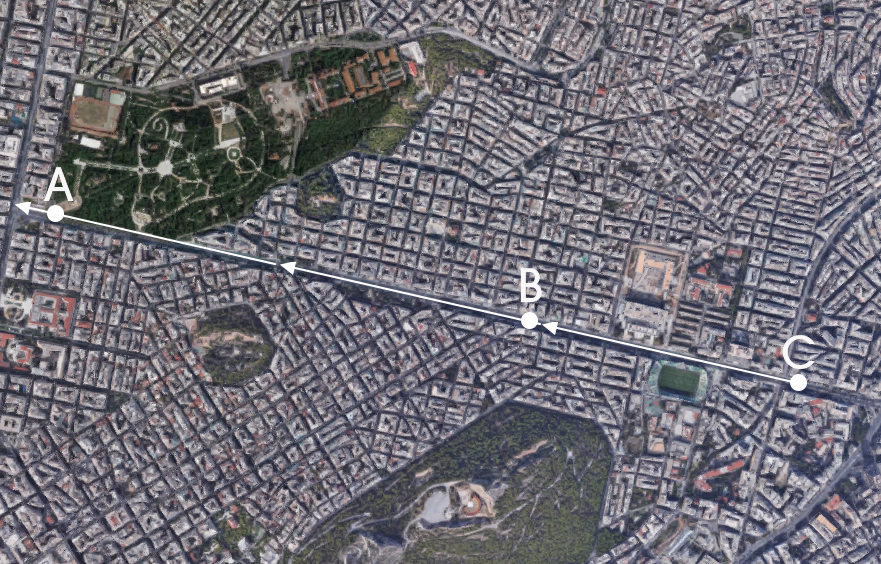
\includegraphics[width=\textwidth]{TrafficMap}
\label{fig:trafficdatamap}
\end{figure}

Analyzing the raw traffic occupancy from an urban network measured on the 90s interval becomes problematic due to the large amount of noise seen at high resolutions \citep{Vlahogianni2014}. Temporal aggregation to larger intervals i.e. 15 min has been practiced over the years as a smoothing technique prior to modeling. Not only does this practice make short-term forecasting irrelevant with today's technology but diminishes useful long memory, nonlinear, and heteroskedastic dynamics in the underlying signal \cite{Vlahogianni2011}.Rather than modeling across different levels of temporal aggregation, as seen in \cite{Shang2006}, we average to 3 minute intervals resulting in 480 daily time points per location. 

Define random variable $O_{L,t}$ as the traffic occupancy for location $L \in\{A,B,C\}$ at time $t$. The lower case representation $o_{L,t}$ represents the known realization of traffic occupancy for location $L$ at time $t$. As common practice, we ignore traffic occupancy data on weekends. Cyclical human behavior patterns throughout the work week lead to weekly seasonal traffic patterns. Data during April 2000 covers four complete weeks. Figure \ref{fig:OrigPlotTrafficOcc} organizes the three occupany time series by day of the week. The first three weeks of the month comprise the training period used to fit the data, and the last week of the month is held out as an evaluation period. The modeling methods require an additional split of the training period. The first two weeks of the training period are designated for model estimation while the last week is used for model selection.

\begin{figure}[!h]
\caption{Traffic Occupancy for Locations A(\textit{maroon}), B(\textit{black}), and C(\textit{blue}) Organized by Day of the Week Measured on 3-Minute Interval }
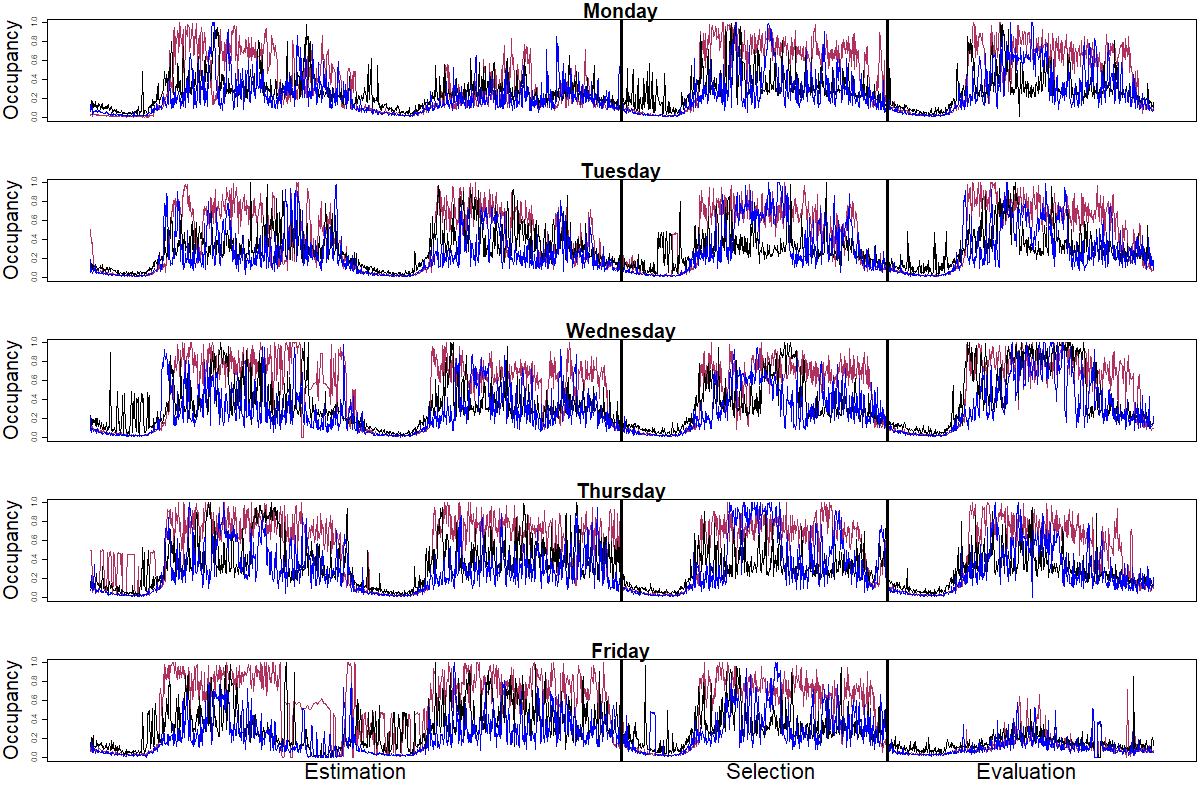
\includegraphics[width=\textwidth]{OrigPlotTrafficOcc}
\label{fig:OrigPlotTrafficOcc}
\end{figure}







%%%%%%%%%%%%%%%%%%%%%%%%%%%%%%%%%%%%%%%%%%%%%%%%%%%%%%%%%%%%%
\section{MODELS}
\label{sec:models}
For each day of the week $D\in\{M,T,W,Th,F\}$ and forecasting horizon $h \in \{1,3,5\}$ , we aim to fit and validate $(D,h)$-specific models to obtain forecast $\widehat{O}_{B,t}=E[O_{B,t}|\mathcal{I}_t]$ where $\mathcal{I}_t=\{o_{A,k},o_{B,k},o_{C,k}|k\in\{t-h,t-h-1,\cdots,t-h-P+1\}$.  The chosen horizons  $h \in \{1,3,5\}$ correspond to 3-minute, 9-minute, and 15-minute forecasts. The additional parameter $P\in\mathbb{N}$ represents the maximum number of lags considered across locations A,B, and C. To control the parameter dimensionality, we fix $P=7$ corresponding to 21 minutes of known information across the traffic network. 

Acknowledging spatio-temporal dependencies downstream and upstream aids in modeling occupancy for a specific loop detector in a fluid traffic network\citep{Kamarianakis2005,Min2010,Min2011,Stathopoulos2003}.The weekly periodicity of traffic occupancy modeled in \cite{Williams1999,Ghosh2007,Kamarianakis2010} and visually seen in Figure \ref{fig:OrigPlotTrafficOcc} defends $D$-specific modeling. Different models designed for each horizon allow for quick, easy multi-step forecasting for practitioners. Especially for nonlinear models, the ``iterative'' approach to obtain unbiased forecast distributions at long horizons from a single model is a slow process involving Monte-Carlo or Bootstrap concepts \citep{Peguin1994,Lundbergh2002}. \cite{Marcellino2006} provide a reasonable argument for ``iterative'' over ``direct''; however, the inclusion of temporal information from nearby locations further complicates the ``iterative'' procedure.

Using function $\phi(x):(0,1)\to\mathbb{R}$ such that $\phi(x)=\log [x/(1-x)]$, we define a new logit transformed variable $Y_{L,t}=\phi(O_{L,t})$. The true variable occupancy resides on the more inclusive $[0,1]$ interval. Values at the boundaries are extremely rare after 3-min temporal aggregation. Recoding $0$ with $0.0001$ and $1$ with $0.9999$ is a nonevasive technique to handle traffic occupancy prior to transformation. If boundary values were more prevalent or provided evidence of important latent effects, we could operate our modeling under a $[0,1]$-inflated distribution. All time series models are defined using the new variables $Y_{A,t}$, $Y_{B,t}$, and $Y_{C,t}$, an approach used for proportional time series since \cite{Wallis1987}. 

\subsection{BASELINE MODELS}

\subsubsection{HORIZON SPECIFIC RANDOM WALKS ($\mathcal{W}(D,h)$)}
The most naive method to obtain an $h$-step ahead forecast $\widehat{Y}_{B,t}$ is with the last known observation $Y_{B,t-h}$. The $h$-specific random walk model in Equation \ref{eq:rwh} does not require any estimation. If a random walk efficiently forecasts traffic occupancy, more complicated modeling schemes become inappropriate for an ATMS striving for urgency.
\begin{equation}
\label{eq:rwh}
Y_{B,t}=Y_{B,t-h}+\epsilon_t
\end{equation}

\subsubsection{HARMONIC SEASONAL PROFILE ($\mathcal{S}_L(D)$)}
Seasonal models allow us to understand the long-run relationship of a variable over time through repetitive cycles. It is common practice in time series analysis to deseasonalize data prior to model buiding through smoothing or seasonal differencing. In many studies, seasonal autoregressive integrated moving average models (SARIMA) have been used to analyze traffic characteristics \citep{Williams2003, Ghosh2005, Zhang2011}. As detailed in \cite{Kumar2015}, these models require large databases of historical data to capture seasonal phenomenon. Similar to \cite{Kumar2015}, we are operating under 3 day period for model training. From a similar dataset, \cite{Kamarianakis2010} used a smoothing spline with 150 degrees of freedom to magnify weekly seasonal patterns and identify structural changes. Smoothing approaches can lead to simple models that can forecast at all horizons.

We expose the daily periodic signal using a harmonic regression model. Harmonic regression estimates a periodic signal from a linear regression over a Fourier basis \citep{Metcalfe2009}. For 3-min data, the seasonal period has a length of 480 discrete measures. Using harmonic regression, we estimate seasonal profiles of $Y_{L,t}$ at all three locations $L \in \{A,B,C\}$.  As expressed in Equation \ref{eq:seas}, we consider a harmonic seasonal model containing the first $H$ terms of the Fourier series.  This model is not considered a baseline model for its simplicity in estimation but for its simplicity in multistep forecasting at all horizons. Notate $\mathcal{S}_L(D)$ as the baseline seasonal model for $Y_{L,t}$. Since forecasts are obtained for location $B$, we mainly discuss model comparisons to seasonal baseline model $\mathcal{S}_B(D)$.

\begin{equation}
\label{eq:seas}
Y_{L,t}=\mu_{L,t}+\sum\limits_{t=1}^{S} \Big[\alpha_{L,t}\sin\Big(\frac{2\pi t}{480}\Big)+\beta_{L,t}\cos\Big(\frac{2\pi t}{480}\Big)\Big]+\epsilon_{L,t}
\end{equation}

\subsection{MODELS USING LOCAL AND RECENT TRAFFIC OCCUPANCIES}
Define $\bm{Y_{L,t-h}}=[Y_{L,t-h},Y_{L,t-h-1},\cdots,Y_{L,t-h-P+1}]'$. To forecast $Y_{B,t}$, we build models using recent information from the location of interest  $\bm{Y_{B,t-h}}$, the location downstream $\bm{Y_{A,t-h}}$, and the location upstream $\bm{Y_{C,t-h}}$ up to maximum lag order P. 

\subsubsection{LINEAR MODEL ($\mathcal{L}_1(D,h)$)}
Under the current setting, the most obvious model is the linear autoregressive distributed lag (ARDL) model seen in Equation \ref{eq:ardl1}. We operate under the assumption that $\epsilon_t \overset{iid}\sim N(0,\sigma^2)$ implying homoskedasticity. Historically, ARDL models have been used to explain long run relationships between time series through distributing the effect of input time series $x_t$ on output time series $y_t$ across lagged terms, even when both time series are cointegrated  \citep{Pesaran1998,Hassler2006}.
\begin{equation}
\label{eq:ardl1}
Y_{B,t}=\mu+\bm{\alpha}'\bm{Y_{A,t-h}}+\bm{\beta}'\bm{Y_{B,t-h}}+\bm{\gamma}'\bm{Y_{C,t-h}}+\epsilon_t
\end{equation}

\subsubsection{NONLINEAR REGIME-SWITCHING MODEL  ($\mathcal{R}_1(D,h)$)}
Dynamical \citep{Queen2009} and volatility changes \citep{Vlahogianni2011} in traffic data decrease the effectiveness of basic time series models \citep{Vlahogianni2004}. Many variants of neural networks were the earliest attempts to capturing the nonlinear dynamics inherent to traffic flow data \cite{Smith1997}. Practical justification popularized neural nets, making them an industry standard technique \citep{Ledoux1997}. For a while, traffic data analysts have filtered traffic data through a prism to understand dynamics through different regimes. Given the regimes, forecasting techniques can be tailored specifically to the current traffic state\citep{Danech1991,Voort1996}. \cite{Zhu2012} defined five states of traffic flow: light, stable, increasing, congested, decreasing. \cite{Xu2012}, then later\cite{Theofilatos2017},  identified nine distinct regimes based on local traffic occupancy to understand accident likelihood.
 
Regime-switching traffic models not only help in cluster identification\citep{Kamarianakis2010,Kamarianakis2012} but also in  regime-based forecasting\citep{Dunne2012}. Combining the self-exciting threshold autoregressive (SETAR) model of \cite{Ghaddar1981} with the linear ARDL model in Equation \ref{eq:ardl1} results in the nonlinear SETARDL model in Equation \ref{eq:setardl1}. The term ``self-exciting'' implies that regime changes are based on recent knowledge about the modeled time series. This model is characterized by abrupt transitions from an ARDL model under low occupancy to a different ARDL model under high occupancy as $Y_{B,t}$ fluctuates around threshold parameter $\delta$.  Assuming $\epsilon_{t,L} \overset{iid}\sim N(0,\sigma_L^2)$ and $\epsilon_{t,H} \overset{iid}\sim N(0,\sigma_H^2)$ permits heteroskedasticity.

Multiple regimes can be identified through additional threshold parameters. In \cite{Kamarianakis2010}, 2-regime to 4-regime models are considered. Bayesian estimation of  3-regime SETARDL model for $Y_{B,t}$ was attempted. Analysis of MCMC chains showed convergence of posterior means for threshold parameters $\delta_1$ and $\delta_2$. When $\delta_1=\delta_2$, the 3-regime SETARDL model effectively simplifies to Equation \ref{eq:setardl1}.
\begin{equation}
\label{eq:setardl1}
Y_{B,t}=
  \begin{cases}
    \mu_L+\bm{\alpha_L}'\bm{Y_{A,t-h}}+\bm{\beta_L}'\bm{Y_{B,t-h}}+\bm{\gamma_L}'\bm{Y_{C,t-h}}+\epsilon_{t,L} & \textrm{ if } Y_{B,t-h}<\delta \\
    \mu_H+\bm{\alpha_H}'\bm{Y_{A,t-h}}+\bm{\beta_H}'\bm{Y_{B,t-h}}+\bm{\gamma_H}'\bm{Y_{C,t-h}}+\epsilon_{t,t-h} & \textrm{ if } Y_{B,t-h}>\delta \\
  \end{cases}
\end{equation}

\subsection{MODELS USING DEVIATIONS FROM SEASONAL PROFILES}
The previous models in Equations \ref{eq:ardl1}-\ref{eq:setardl1} ignore daily seasonality. Suppose $\widehat{Y}_{L,t}$ is the posterior expectation on location $L$ at time $t$ from the seasonal model in Equation \ref{eq:seas}. The newly defined  $\Delta_{L,t}=Y_{L,t}-\widehat{Y}_{L,t}$ is interpreted as a deviation from the seasonal profile for location $L$ at time $t$. At time $t$, the vector $\bm{\Delta_{L,t-h}}=[\Delta_{L,t-h},\Delta_{L,t-h-1},\cdots,\Delta_{L,t-h-P+1}]'$ represent the last $P$ known deviations from the seasonal profile at location $L$. The next two models attempt to find underlying short run relationships between seasonally adjusted time series at all three locations.

Often, seasonal adjustment means seasonal differencing. Since weekday traffic occupancy clearly exhibits weekly patterns, harmonic regression analysis has value for understanding average behavior for a particular day. Diversions of traffic occupancy away from average behavior indicate future diversions.  Equations \ref{eq:ardl2}-\ref{eq:setardl2} are ARDL and SETARDL models applied to the deviations from seasonal profiles. For consistency, regime changes in Equation \ref{eq:setardl2} are based on $Y_{B,t-h}$. Horizon-specific forecasts of $Y_{B,t}$ from these models are easily obtained by adding the fitted seasonal component to the forecasted deviation. 

\subsubsection{LINEAR MODEL ($\mathcal{L}_2(D,h)$)}
\begin{equation}
\label{eq:ardl2}
\Delta_{B,t}=\mu+\bm{\alpha}'\bm{\Delta_{A,t-h}}+\bm{\beta}'\bm{\Delta_{B,t-h}}+\bm{\gamma}'\bm{\Delta_{C,t-h}}+\epsilon_t
\end{equation}

\subsubsection{NONLINEAR REGIME-SWITCHING MODEL ($\mathcal{R}_2(D,h)$)}
\begin{equation}
\label{eq:setardl2}
\Delta_{B,t}=
  \begin{cases}
    \mu_L+\bm{\alpha_L}'\bm{\Delta_{A,t-h}}+\bm{\beta_L}'\bm{\Delta_{B,t-h}}+\bm{\gamma_L}'\bm{\Delta_{C,t-h}}+\epsilon_{t,L} & \textrm{ if } Y_{B,t-h}<\delta \\
    \mu_H+\bm{\alpha_H}'\bm{\Delta_{A,t-h}}+\bm{\beta_H}'\bm{\Delta_{B,t-h}}+\bm{\gamma_H}'\bm{\Delta_{C,t-h}}+\epsilon_{t,t-h} & \textrm{ if } Y_{B,t-h}>\delta \\
  \end{cases}
\end{equation}








%%%%%%%%%%%%%%%%%%%%%%%%%%%%%%%%%%%%%%%%%%%%%%%%%%%%%%%%%%%%
\section{ESTIMATION, DISCRIMINATION, AND SELECTION}
\label{sec:bayesest}
In Section \ref{sec:models}, we presented the following $(D,h)$-specific models: $\mathcal{W}(D,h)$, $\mathcal{S}_B(D)$, $\mathcal{L}_1(D,h)$, $\mathcal{R}_1(D,h)$, $\mathcal{L}_2(D,h)$, and $\mathcal{R}_2(D,h)$. Models $\mathcal{W}(D,h)$ and $\mathcal{S}_B(D)$ are set aside for baseline comparisons. Given day $D$ and forecasting horizon $h$, full model $\mathcal{M} \in \{L_1(D,h),R_1(D,h),L_2(D,h),R_2(D,h)\}$ is fully defined by a corresponding parameter vector $\bm{\theta}_{\mathcal{M}}\in \bm{\Theta}_\mathcal{M}$. For all $\mathcal{M}$, the dimensionality $\dim(\bm{\Theta}_\mathcal{M})$ increases with order $P$. Furthermore, the number of harmonic frequencies $S$ considered in $\mathcal{S}_B(D)$ increases the $\dim(\bm{\Theta}_\mathcal{M})$ for $\mathcal{L}_2(D,h)$ and $\mathcal{R}_2(D,h)$. Table \ref{tab:dimtheta} summarizes the size of the parameter space of each full model for fixed $S$ and $P$.

\begin{table}[!h]
  \footnotesize
  \centering
  \caption{Dimensionality of Parameter Space $\bm{\Theta}$ For Fixed $P$ and $S$ }
    \begin{tabular}{cc}
    \toprule
   Model & $\dim(\bm{\Theta})$  \\
    \midrule
    $\mathcal{W}(D,h)$ & $1$ \\
    $\mathcal{S}_B(D)$ & $2H+2$ \\
    $\mathcal{L}_1(D,h)$ & $3P+1+1=3P+2$ \\
    $\mathcal{R}_1(D,h)$ & $2(3P+2)=6P+4$ \\
    $\mathcal{L}_2(D,h)$ & $3(2H+2)+ 3P+2=6H+3P+8$ \\
    $\mathcal{R}_2(D,h)$ & $3(2H+2)+6P+4=6H+6P+10$ \\
    \bottomrule
    \end{tabular}%
  \label{tab:dimtheta}%
\end{table}%

Bayesian inference is the process of updating the assumed prior distribution $\bm{\theta}_{\mathcal{M}}\sim f(\bm{\theta}_{\mathcal{M}})$ to an informed posterior distribution $\bm{\theta}_\mathcal{M}|\mathcal{I} \sim f(\bm{\theta}_\mathcal{M}|\mathcal{I})$ upon realizations  $\mathcal{I}=\{y_{A,t},y_{B,t},y_{C,t}|t \in \{1,2,\cdots,T\}\}$. Bayes's Law in Equation \ref{eq:bayeslaw} is the probability rule that drives this logic. Credible regions and estimates of $\bm{\theta}_\mathcal{M}$ are determined from $f(\bm{\theta}_\mathcal{M}|\mathcal{I})$ directly or via posterior sampling from $f(\bm{\theta}_\mathcal{M}|\mathcal{I})$. Typically, variations of Markov chain Monte Carlo (MCMC) algorithms are used for the latter.
\begin{equation}
\label{eq:bayeslaw}
\begin{split}
	f(\bm{\theta}_\mathcal{M}|\mathcal{I})&=\frac{f(\bm{\theta}_\mathcal{M},\mathcal{I})}{f(\mathcal{I})}=\frac{f(\mathcal{I}|\bm{\theta}_\mathcal{M})f(\bm{\theta}_\mathcal{M})}{f(\mathcal{I})}\\
	& \propto f(\mathcal{I}|\bm{\theta}_\mathcal{M})f(\bm{\theta}_\mathcal{M})=(Likelihood)(Prior)\\
\end{split}
\end{equation}

Bayesian time series analysis is not exempt to model misspecification, specifically as it relates to $P$ and $S$.   Although inference about $\bm{\theta}_\mathcal{M}$ is important, the primary focus is on forecasting $y_{B,t+h}$ given known $\mathcal{I}$. All interest pertaining to $\bm{\theta}_\mathcal{M}$ is strictly tied to  understanding the posterior predictive distribution $f(y_{B,t+h}|\mathcal{I})=\int_{\bm{\Theta}} f(y_{B,t+h}|\bm{\theta}_\mathcal{M})f(\bm{\theta}_\mathcal{M}|\mathcal{I}) d\bm{\theta}_\mathcal{M}$. 

Without loss of generality, consider the linear AR($P$) and nonlinear TAR($P$) models specified in Equations \ref{eq:genlin}-\ref{eq:gentar} and abbreviated $\mathcal{M}_L$ and $\mathcal{M}_R$, respectively.
\begin{equation}
\label{eq:genlin}
\begin{split}
y_t&=\alpha_0+\alpha_1y_{t-1}+\alpha_2y_{t-2}+\cdots+\alpha_Py_{t-P}+\epsilon_t \\
y_t&=\bm{\alpha}'\bm{y_{t-1}}+\epsilon_t 
\end{split}
\end{equation}
\begin{equation}
\label{eq:gentar}
\begin{split}
y_t&=
  \begin{cases}
    \alpha_0+\alpha_1y_{t-1}+\alpha_2y_{t-2}+\cdots+\alpha_Py_{t-P}+\epsilon_{\alpha,t} & \textrm{ if } z_t<\delta \\
    \beta_0+\beta_1y_{t-1}+\beta_2y_{t-2}+\cdots+\beta_Py_{t-P}+\epsilon_{\beta,t} & \textrm{ if } z_t>\delta \\
  \end{cases}\\
  &=
    \begin{cases}
    \bm{\alpha}'\bm{y_{t-1}} +\epsilon_{\alpha,t} & \textrm{ if } z_t<\delta \\
     \bm{\beta}'\bm{y_{t-1}} +\epsilon_{\beta,t} & \textrm{ if } z_t>\delta \\
  \end{cases}\\
  \end{split}
\end{equation}

Bayesian model selection of time series often defaults to posterior estimation of $P$. For both $\mathcal{M}_L$ and $\mathcal{M}_R$, various ways of handling the uncertainty about $P$ have been proposed. Consider $P \in \bm{\theta}$. The reversible jump MCMC (RJMCMC) algorithm of \cite{Green1995} modifies $\dim(\bm{\Theta})$ with posterior sampling of $P$. Exploiting the constant expansion and contraction of the parameter space results in an efficient method for order selection in both linear \citep{Troughton1997,Vermaak2004} and nonlinear \citep{Campbell2004,Lopes2006} time series models. In all traffic models presented, we include $P$ lagged traffic occupancies from all three locations. RJMCMC could be applied to these models but would be inflexible. If traffic models with a different number of lags for the three locations are considered, then the simplicity of RJMCMC is lost. 

Besides the issues with RJMCMC, operating under the assumption that model complexity is fully determined by $P$ fails to detect insignificant lagged terms in the middle. In more complex urban traffic networks, information at many locations may be useful but at different times depending on the distance and level of congestion. For our methods, we interpret $P$ as the maximum lag order considered for all endogenous and exogenous time series. The choice of $P$ \textit{a priori} is intentionally overestimated to allow Bayesian subset selection and/or Bayesian shrinkage to adapt to more parsimonious options. Bayesian subset selection \citep{George1993,Kuo1998,Chipman2001,Dellaportas2002} and shrinkage methods \citep{Park2008,Carvalho2009,Armagan2013,Bhattacharya2015} have been heavily developed through disjointed research. An abridgment of these topics are found in \cite{OHara2009}. Recently, bridges have developed between shrinkage and model selection to utilize the computational efficiency of shrinkage for the attainment of an interpretable, reduced model.  \citep{Lykou2013,Hahn2015,Rockova2016}.

Next, we outline a three step Bayesian procedure combining Bayesian shrinkage with projection predictive variable selection for the general nonlinear TAR($P$) model $\mathcal{M}_R$. \cite{vehtari2012,Piironen2015,Piironen2017}  illustrated the efficacy of this approach in linear Gaussian models for cross-sectional data. For this reason, we present the procedures for the nonlinear case only. The conditional linear nature of $\mathcal{M}_R$  allows us to perform regime-specific regularization and model selection. Where cross-validation was used in \cite{Piironen2015,Piironen2017}, final model selection is based on forecasting accuracy.


\subsection{BAYESIAN SHRINKAGE ESTIMATION}
Bayesian shrinkage is characterized by continuous prior specifications expressed through scale mixture of normal distributions, dating back to\cite{Andrews1974} and \cite{West1987}.  Bayesian LASSO (BLASSO) \citep{Yuan2005,Park2008,Hans2009,Hans2010,Rajaratnam2015} applied a $double-exponential$ prior specification to mimic the $L1$-regularization of \cite{Tibshirani1994}, while the Bayesian horseshoe (BHS)  \cite{Carvalho2009,Carvalho2010} hinges on a $half-cauchy$ hierarchy.  Of the broad class of global-local shrinkage priors \citep{Polson2010}, BLASSO and BHS have become the most popular choices. As noted in \cite{Bhadra2017}, recent computational developments and modifications in BHS have led to fast sampling algorithms and better handling of high-dimensional scenarios \citep{Bhadra2016,Makalic2016b}.  Similar to the LASSO of \cite{Tibshirani1994}, the combination of parameter shrinkage and selection makes BLASSO an enticing pick. As we often see in time series modeling, high-dimensionality is usually not the problem. Typically, models can be expressed using a few lags; therefore, not many are considered. The major issue with the ARDL($P$) and SETARDL($P$) models is the inherent multicollinearity existent in the covariates. As discussed in \cite{Friedman2001,Zou2005,Mallick2013}, LASSO-type penalization typically stumbles in the presence of multicollinearity. Purposefully, we adapt BHS for initial sparse estimation of autoregressive coefficients under the full model.

The full TAR($P$) model $\mathcal{M}_R$ is defined by parameter vector $\bm{\theta}_{\mathcal{M}_R}=[\bm{\alpha},\bm{\beta},\delta,\sigma_\alpha,\sigma_\beta]'$. If the threshold $\delta$ is known, $\mathcal{M}_R$ becomes a linear model conditional on $z_t$. If $z_t<\delta$, $y_t=\bm{\alpha}'\bm{y_{t-1}}+\epsilon_{\alpha,t}$, and if $z_t<\delta$, $y_t=\bm{\beta}'\bm{y_{t-1}}+\epsilon_{\beta,t}$. For future reference, we abbreviate the low-regime model $\mathcal{M}_{LR}$ and the high-regime model $\mathcal{M}_{HR}$.

Posterior sampling from $f(\bm{\theta}_{\mathcal{M}_R}|\mathcal{M}_R,\mathcal{I})$ revolves around a combination of Gibbs sampling \citep{Gelfand1990} for regime specific parameters $\bm{\alpha}$, $\bm{\beta}$, $\sigma_\alpha$, and $\sigma_\beta$, and Metropolis-Hastings \citep{Metropolis1953,Hastings1970} for the threshold $\delta$  \citep{Geweke1993,Chen1998,Koop1999,Campbell2004}. Aligning with previous research, diffuse inverse gamma priors will be used for $\sigma_\alpha$ and $\sigma_\beta$. To ensure each regime is represented by at least 15\% of the data, $\delta\sim U(q_{Z}(0.15),q_Z(0.85))$ where $q_Z(.)$ is the empirical quantile function for transition variable Z.

Bayesian variable shrinkage and selection specifically targets the non-intercept parameters in $\bm{\alpha}$ and $\bm{\beta}$. Noninformative $Normal$ priors are used for regime intercepts $\alpha_0$ and $\beta_0$, while the hierarchical representation of the horseshoe prior, expressed in Equation \ref{eq:hsp} is used for the coefficients. In this representation, $C^+$ symbolizes $half-Cauchy$ distribution. The Bayesian horseshoe hierarchy is defined within the models $\mathcal{M}_{LR}$ and $\mathcal{M}_{HR}$ via  regime-specific global shrinkage parameters $\lambda_\alpha$ and $\lambda_\beta$. 
\begin{equation}
\label{eq:hsp}
\begin{split}
 	\alpha_j &\sim N(0,\lambda^2_{\alpha_j}\lambda_{\alpha}^2), \textrm{ } \lambda_{\alpha_j}\sim C^+(0,1), \textrm{ } \lambda_\alpha \sim C^+(0,1) \\
 	\beta_j & \sim N(0,\lambda^2_{\beta_j}\lambda_{\beta}^2), \textrm{ } \lambda_{\beta_j}\sim C^+(0,1), \textrm{ } \lambda_\beta \sim C^+(0,1)\\
 	& \forall j \in \{1,2,3,\cdots,P\}
\end{split}
\end{equation}

Posterior sampling under these prior specifications is easily conducted using popular Bayesian software packages. The smooth integration of JAGS \cite{Plummer2003} with R makes JAGS our favored option for MCMC. JAGS model code for Bayesian horseshoe estimation of both linear and nonlinear models is provided in the appendix. To capture convergence, multiple chains with different starting values are constantly assessed. Posterior samples prior to convergence are dropped and effective sample size is measured to ensure posterior quantiles can be adequately assessed.

\subsection{KULLBACK-LEIBLER DISCRIMINATION}
The joint posterior distribution $f(\bm{\theta}_{\mathcal{M}_R}|\mathcal{M}_R,\mathcal{I})$ obtained through BHS priors is  a good starting point. Although BHS priors separately invoked on $\bm{\alpha}$ and $\bm{\beta}$ lead to regime-specific sparse estimation, it is unlikely posterior means $E[\bm{\alpha}|\mathcal{M}_R,\mathcal{I}]$ and $E[\bm{\beta}|\mathcal{M}_R,\mathcal{I}]$ contain true $0$ values.   Assuming the data follows some TAR process, the model space containing all submodels of $\mathcal{M}_R$ contains $2^{2(P+1)}$ different alternatives. Naively exploring this model space to find the best reduced model $\mathcal{M}^*_R$ is an inefficient approach.

The Kullback-Leibler (KL) divergence is an asymmetric measure of distance between two probability distributions\citep{Kullback1951}. \cite{burnham2003} provides a nice discussion connecting KL divergence to subset model selection based on Aikaike information criteria (AIC). \cite{Goutis1998} and \cite{Dupuis2003} use KL divergence to compare a proposed submodel to a larger reference model based on conditional likelhoods. If minor discrepancy is detected between the reference model and a particular submodel, the simpler submodel can be considered. The proposed method derives a posterior distribution for a submodel through projection from the information in the sampled posterior distribution for the larger reference model. \cite{Piironen2017} provided analytical solutions to obtain the projected parameters and evaluate the resulting KL divergence for Gaussian linear models. For $\mathcal{M}_R$, we treat $\mathcal{M}_{LR}$ and $\mathcal{M}_{HR}$ as reference models for the corresponding regimes. Both $\mathcal{M}_{LR}$ and $\mathcal{M}_{HR}$ are conditionally linear Gaussian models; therefore we extend the methods of \cite{Piironen2017} to the general TAR($P$). 

Let $\bm{Y_{t-1}}$ be the $T\times(P+1)$ matrix where the $k$th row is the vector of lagged information $\bm{y_{k-1}}'=[1,y_{k-1},y_{k-2},\cdots,y_{k-P}]$. We define $\bm{\theta}^{(s)}$ as the $s$th posterior draw from $f(\bm{\theta}_{\mathcal{M}_R}|\mathcal{M}_R,\mathcal{I})$ partitioned by $[\bm{\alpha}^{(s)},\sigma_\alpha^{(s)},\bm{\beta}^{(s)},\sigma_\beta^{(s)},\delta^{(s)}]$. Now, consider an arbitrary submodel $\mathcal{M}^\perp_{R}$ characterized by  $\mathcal{M}^\perp_{LR}$ and $\mathcal{M}^\perp_{HR}$. Similarly, define the $s$th draw from the posterior $f(\bm{\theta}_{\mathcal{M}^\perp_R}|\mathcal{M}^\perp_R,\mathcal{I})$  as $\bm{\theta}^{\perp(s)}=[\bm{\alpha}^{\perp(s)},\sigma_\alpha^{\perp(s)},\bm{\beta}^{\perp(s)},\sigma_\beta^{\perp(s)},\delta^{(s)}]$.  
 
Given $\bm{\theta}^{(s)}$, we start by splitting model matrix $\bm{Y_{t-1}}$ into two smaller matrices $\bm{Y_{LR,t-1}}$ and $\bm{Y_{HR,t-1}}$ based on the sampled threshold $\delta^{(s)}$. $\bm{Y_{LR,t-1}}$ contains the rows of $\bm{Y_{t-1}}$ corresponding to the times whenever $z_t<\delta$, and $\bm{Y_{HR,t-1}}$ contains the rows of  $\bm{Y_{t-1}}$ not contained in $\bm{Y_{LR,t-1}}$. Furthermore, $\bm{Y^{\perp}_{LR,t-1}}$ and $\bm{Y^{\perp}_{HR,t-1}}$ contain the columns of $\bm{Y_{LR,t-1}}$ and $\bm{Y_{HR,t-1}}$ reflective of the proposed regime-specific submodels $\mathcal{M}^\perp_{LR}$ and $\mathcal{M}^\perp_{HR}$, respectively. For each $s \in \{1,2,\cdots,S\}$, we sample $\bm{\theta}^{\perp(s)}$ from the  projected posterior $f(\bm{\theta}_{\mathcal{M}^\perp_R}|\mathcal{M}^\perp_R,\mathcal{I})$ by applying Equation \ref{eq:proj} to the original $\bm{\theta}^{(s)}$ drawn under BHS priors.
\begin{equation}
\label{eq:proj}
\begin{split}
\bm{\alpha}^{\perp(s)}&=(\bm{Y^{\perp'}_{LR,t-1}}\bm{Y^{\perp}_{LR,t-1}})^{-1} \bm{Y^{\perp'}_{LR,t-1}}     \bm{Y_{LR,t-1}}\bm{\alpha}^{(s)}\\
\sigma_\alpha^{\perp(s)}&=\sqrt{\sigma_\alpha^{(s)}+\frac{( \bm{Y_{LR,t-1}}\bm{\alpha}^{(s)}-\bm{Y^\perp_{LR,t-1}}\bm{\alpha}^{\perp(s)})'( \bm{Y_{LR,t-1}}\bm{\alpha}^{(s)}-\bm{Y^\perp_{LR,t-1}}\bm{\alpha}^{\perp(s)})}{T}                                  }\\
\bm{\beta}^{\perp(s)}&=(\bm{Y^{\perp'}_{HR,t-1}}\bm{Y^{\perp}_{HR,t-1}})^{-1} \bm{Y^{\perp'}_{HR,t-1}} \bm{Y_{HR,t-1}}\bm{\beta}^{(s)}\\
\sigma_\beta^{\perp(s)}&=\sqrt{\sigma_\beta^{(s)}+\frac{( \bm{Y_{HR,t-1}}\bm{\beta}^{(s)}-\bm{Y^\perp_{HR,t-1}}\bm{\beta}^{\perp(s)})'( \bm{Y_{HR,t-1}}\bm{\beta}^{(s)}-\bm{Y^\perp_{HR,t-1}}\bm{\beta}^{\perp(s)})}{T}                                   }
\end{split}
\end{equation}

For each posterior draw from $f(\bm{\theta}_{\mathcal{M}_R}|\mathcal{M}_{R},\mathcal{I})$, we measure the corresponding regime-specific KL divergences $d_{LR}$ and $d_{HR}$ using Equation \ref{eq:klds}.
\begin{equation}
\label{eq:klds}
\begin{split}
d^{(s)}_{LR}(\bm{\alpha}^{(s)},\sigma^{(s)}_\alpha)&=\frac{1}{2}\log\bigg(\frac{\sigma^{\perp(s)}_\alpha}{\sigma^{(s)}_\alpha}\bigg)\\
d^{(s)}_{HR}(\bm{\beta}^{(s)},\sigma^{(s)}_\beta)&=\frac{1}{2}\log\bigg(\frac{\sigma^{\perp(s)}_\beta}{\sigma^{(s)}_\beta}\bigg)
\end{split}
\end{equation}

Finally, measures $D(\mathcal{M}_{LR}||\mathcal{M}^\perp_{LR})$ and $D(\mathcal{M}_{HR}||\mathcal{M}^\perp_{HR})$ expressed in Equation \ref{eq:disc} determine the discrepancy between regime-specific full models to proposed reduced versions. 
\begin{equation}
\label{eq:disc}
\begin{split}
D(\mathcal{M}_{LR}||\mathcal{M}^\perp_{LR})&=\frac{1}{S}\sum\limits^S_{s=1} d^{(s)}_{LR}(\bm{\alpha}^{(s)},\sigma^{(s)}_\alpha)    \\
D(\mathcal{M}_{HR}||\mathcal{M}^\perp_{HR})&=\frac{1}{S}\sum\limits^S_{s=1} d^{(s)}_{HR}(\bm{\beta}^{(s)},\sigma^{(s)}_\beta)     \\
\end{split}
\end{equation}

Using these concepts, we avoid surveying the entire  $2^{2(P+1)}$ model space by employing a forward stepwise selection algorithm to identify the best regime-specific submodel at every possible level of flexibility bounded by predetermined $P$. The simplest models considered are the intercept-only models denoted $\mathcal{M}^0_{LR}$ and $\mathcal{M}^0_{HR}$. The initial discrepancies  $D(\mathcal{M}_{LR}||\mathcal{M}^0_{LR})$ and $D(\mathcal{M}_{HR}||\mathcal{M}^0_{HR})$ represent the maximum divergence between the full models and all possible submodels. 

For each level of flexibility $p \in \{1,2,\cdots,P\}$, we find the best regime-specific submodels $\mathcal{M}^p_{LR}$ and $\mathcal{M}^p_{HR}$. Starting with $p=1$, we consider all two dimensional submodels including the intercept and one lagged term. $\mathcal{M}^1_{LR}$ and $\mathcal{M}^1_{HR}$ are chosen based on minimized discrepancy when compared to the full model. Then for $p=2$, all three dimensional regime-specific submodels nesting $\mathcal{M}^1_{LR}$ and $\mathcal{M}^1_{HR}$ are compared to the corresponding full models to find $\mathcal{M}^2_{LR}$ and $\mathcal{M}^2_{HR}$. Continuing this process results in $P+1$ considerations for $\mathcal{M}_{LR}$ and $P+1$ considerations for $\mathcal{M}_{HR}$. 

\subsection{FINAL MODEL SELECTION}
The final reduced models $\mathcal{M}^*_{LR}$ and $\mathcal{M}^*_{HR}$ are chosen from the $2P+2$ options identified through the forward stepwise algorithm. \cite{Dupuis2003} utilized the additive properties of KL divergence for nested models to choose the best model based on relative explanatory power defined in Equation \ref{eq:rep}. As $p$ goes from $0$ to $P$, RelE strictly increases from 0 to 1. As noted by \cite{Dupuis2003} and \cite{Piironen2017}, $\mathcal{M}^*_{LR}$ and $\mathcal{M}^*_{HR}$ can be the smallest submodels that achieve a $RelE > E^*$, where $E^*$ is a predetermined threshold. It is recommended $E^*$ be large i.e. $>90\%$.
\begin{equation}
\label{eq:rep}
\begin{split}
RelE(\mathcal{M}^p)&=1-\frac{D(\mathcal{M}||\mathcal{M}^p)}{D(\mathcal{M}||\mathcal{M}^0)}\\
\end{split}
\end{equation}

\cite{Piironen2015,Piironen2017} favors final selection based on out-of-sample prediction. Regarding time series models, this implies forecasting performance. We choose the final regime-specific reduced models $\mathcal{M}^*_{LR}$ and $\mathcal{M}^*_{HR}$ based on the minimization of  regime-specific root mean squared forecast error (RMSFE) over a time period intentionally left out. The formula for RMSFE is stated in \ref{eq:rmsfe1}.
\begin{equation}
 	\label{eq:rmsfe1}
  RMSFE(\mathcal{M}^p)=\sqrt{\frac{1}{T}\sum (y_t-\hat{y}_t)^2}
\end{equation}










%%%%%%%%%%%%%%%%%%%%%%%%%%%%%%%%%%%%%%%%%%%%%%%%%%%%%%%%%%%%%%%%%%%%%%%%
\section{FORECASTING EVALUATION}
Threshold autoregressive models for traffic occupancy are obvious, considering the structural differences between free flow and congested states. Although practice invites these considerations, it is not necessary that TAR models achieve optimal forecasting accuracy over linear models. Even under nonlinear simulated data, \cite{Davies1988} and \cite{Pemberton1989} illustrated that linear models can occasionally achieve equivalent or better forecasting accuracy than nonlinear competitors \citep{Guo1997,Stock1998a,Dacco1999}.

Given arbitrary full model  $\mathcal{M}$, the methods in Section \ref{sec:bayesest} lead us to final submodel $\mathcal{M}^*$. Final selection of $\mathcal{M}^*$ was indicative of optimal forecasting performance at a specific horizon $h$. By design, optimal forecasts and credible regions for $y_{B,t+h}$ are based on the simulated predictive posterior distribution $f_Y(y_{B,t+h}|\mathcal{I})$ defined on $\mathbb{R}$. The inverse logit function $\phi^{-1}(x):\mathbb{R}\to (0,1)$ where $\phi^{-1}(x)=\exp(x)/[1+\exp(x)]$ provides a path from $f_Y(y_{B,t+h}|\mathcal{I})$ to $f_O(o_{B,t+h}|\mathcal{I})$. Let $\widehat{Y}_{B,t+h}=E[Y_{B,t+h}|\mathcal{I}]$. Because $\phi(x)$ is a nonlinear transformation, $\widehat{O}_{B,t+h}=E[O_{B,t+h}|\mathcal{I}] \neq \phi^{-1}(\widehat{Y}_{B,t+h})$. The natural bias and correction method introduced from nonlinear transformations (i.e. general log function) is discussed in \cite{Metcalfe2009}. For $s \in \{1,2,\cdots, S\}$, we simulate $f_O(o_{B,t+h}|\mathcal{I})$ using posterior draws $y^{(s)}_{B,t+h}$ from $f_Y(y_{B,t+h}|\mathcal{I})$. Figure \ref{fig:posttrans} graphically portrays this process.

\begin{figure}[!h]
\label{fig:posttrans}
\caption{Path to Obtain the Posterior Distribution $f_O(o_{B,t+h}|\mathcal{I})$ from the Posterior Distribution  $f_Y(y_{B,t+h}|\mathcal{I})$ Using Monte Carlo Draws}
\centering
\begin{tikzpicture}[line width=1pt,>=latex]
\sffamily
\node (a2) {$y^{(s)}_{B,t+h}$};

\node[right=5cm of a2] (b2) {$o^{(s)}_{B,t+h}$};

\node[shape=ellipse,draw,minimum size=2.5cm,fit={(a2)}] {};
\node[shape=ellipse,draw,minimum size=2.5cm,fit={(b2)}] {};

\node[below=1.25cm of a2,font=\Large\bfseries] {$f_Y(y_{B,t+h}|\mathcal{I})$};
\node[below=1.25cm of b2,font=\Large\bfseries] {$f_O(o_{B,t+h}|\mathcal{I})$};

\draw[->,black] (a2) -- node[label=above:$\phi^{-1}(x)$] {} (b2);
\end{tikzpicture}
\end{figure}

On the original $(0,1)$-interval, we evaluate traffic occupancy forecasts for all full models $\mathcal{M}$ and final models $\mathcal{M}^*$. Monte Carlo methods are utilized to form the posterior predictive distribution  $f_O(o_{B,t+h}|\mathcal{I})$ to obtain point estimates from posterior means and credible regions from posterior quantiles. The last week of April 2000 was intentionally neglected for forecast evaluation. For each $(D,h)$-specific model, we have $n_h=480-h$ time points requiring forecasts. Forecasts for this week are obtained under the assumption that the posterior distribution of $\bm{\theta}_\mathcal{M}$ given the data $\mathcal{I}$ is static throughout the evaluation period. Typically, $f(\bm{\theta}_\mathcal{M}|\mathcal{I})$ can be updated when new information is added to $\mathcal{I}$.

Define $\mathbb{M}=\{L_1(D,h), R_1(D,h), L_2(D,h), R_2(D,h)\}$ to be the set of all full models and $\mathbb{M}^*=\{L^*_1(D,h), R^*_1(D,h), L^*_2(D,h), R^*_2(D,h)\}$ to be the corresponding reduced models. Given day $D$ and horizon $h$, we use three forecast accuracy metrics to answer the following quesions about $\mathbb{M}$ and $\mathbb{M}^*$:    
\begin{itemize}
   \item How do the models compare to each other?
   \item How do the full models compare to the final models?
   \item How do the models compare to benchmark naive and seasonal models?
 \end{itemize}

RMSFE can help answer the first two proposed questions. RMSFE allows the practitioner to understand traffic occupancy forecast error on the original percentage scale. Since RMSFE was used in the selection of $\mathcal{M}^*$,  we continue to apply RMSFE in model evaluation. The formula for RMSFE in terms of traffic occupancy is restated in \ref{eq:rmsfe2}.
\begin{equation}
 	\label{eq:rmsfe2}
  RMSFE(h)=\sqrt{\frac{1}{n_h}\sum\limits_{t=h+1}^{480} (O_{B,t}-\widehat{O}_{B,t})^2}
\end{equation}

Denote the mean absolute error (MAE) from daily baseline models $\mathcal{W}(D,h)$ and $\mathcal{S}_B(D)$ as $\textrm{MAE}_{W}(h)$ and $\textrm{MAE}_{S}$. Relative adaptations of MAE summarize the advantages of using a complex model over a simple benchmark choice \citep{Hyndman2006}. \cite{Theil1966} introduced this concept to random walks for evaluation of 1-step ahead performance. The $h$-specific relative MAFE (RelMAFE(h)) in Equation \ref{eq:relmafe} quantifies the benefit of a $(D,h)$-specific model to a $h$-specific random walk. We further this idea to the seasonal RelMAFE (SRelMAFE) in Equation \ref{eq:srelmafe} to understand advantages over seasonal profiles \citep{Makridakis2008}.
\begin{equation}
\label{eq:relmafe}
  RelMAFE(h)=\frac{1}{n_h}\sum\limits_{t=h+1}^{480}\left|\frac{O_{B,t}-\widehat{O}_{B,t}}{\textrm{MAE}_{W}(h)}\right|
\end{equation}
\begin{equation}
\label{eq:srelmafe}
  SRelMAFE(h)=\frac{1}{n_h}\sum\limits_{t=h+1}^{480}\left|\frac{O_{B,t}-\widehat{O}_{B,t}}{\textrm{MAE}_{S}}\right|
\end{equation}



